\documentclass{beamer}
\usepackage[orientation=landscape,size=a0,scale=2]{beamerposter}
\usepackage[utf8]{inputenc}
\usepackage{amsthm}
\usepackage{mathtools}
\usepackage{amsfonts}
\usepackage{amsmath}
\usepackage{amssymb}
\usepackage{tikz}
\usepackage{float}
% \usepackage{subfloat}
\usepackage{subfig}
\usepackage{graphicx}
%\usepackage{tkz-euclide}
\usetikzlibrary{shapes.geometric, arrows, calc}
\usepackage[style=authoryear]{biblatex}
\addbibresource{export-data.bib}
\nocite{*}

\DeclareMathOperator*{\vv}{\mathbf{v}}
\DeclareMathOperator*{\xx}{\mathbf{x}}
\DeclareMathOperator*{\yy}{\mathbf{y}}
\DeclareMathOperator*{\pp}{\mathbf{p}}

\renewcommand\mathfamilydefault{\rmdefault}

\usepackage{caption}
\captionsetup[figure]{font=normalsize}

% Numbered figures
\setbeamertemplate{caption}[numbered]

\title{You'll never guess how fast these 10 polygons expand!!}
\author{Xiang Cheng, George Ekman, Ziling Hu, Siyuan Lu}
\institute{University of Wisconsin-Madison}
\date{August 2022}

\begin{document}

% THE ACTUAL POSTER
\begin{frame}

% HEADER
{
    {\vspace{-1cm}
    \centering
        \Huge %You'll never guess how fast these polygons expand!! \\
        Carpenter's Rule Problem \& Chord-arc Constant Algorithms \\
    }
    % \vspace{-2cm}
    \begin{columns}
        \column{0.1\textwidth}
            {\centering
            \qquad
            
\includegraphics[height=0.6\textwidth]{figures/uw-crest-web.png}}
            
        \column{0.8\textwidth}
            {\centering
            \Large Xiang Cheng$^1$, George Ekman$^1$, Ziling Hu$^1$, Siyuan Lu$^1$ \\
            \Large Advisor: Jack Burkart$^1$ \\
            \large $^1$Department of Mathematics, University of Wisconsin-Madison \\
            }
            
        \column{0.1\textwidth}
            {%\centering
            \hspace{-2cm}
            
\includegraphics[width=0.6\textwidth]{figures/nsf.png}}
    \end{columns}
}
\vspace{1cm}
\noindent\rule{117cm}{0.4pt}
\vspace{0.01pt}
% BODY
    \begin{columns}[t]
    \column{0.33\textwidth}
        {\centering \large \textbf{Background} \\}
        % \vspace{0.3cm}
        \textbf{Carpenter's Rule Problem:} Can a polygon be expanded into a convex shape without creating intersections or distorting lengths? It turns out, yes! \\
        
        \vspace{1cm}
        Let ${\pp}_i$ be the position of vertex $i$, and ${\vv}_i$ be its velocity. The desired motion is a solution to the optimization problem below, where $E$ is the set of connected pairs and $S$ disconnected pairs:
        \begin{equation*}
            \min \sum_{i \in V} \Vert {\vv}_i \Vert^2 + \sum_{(i,\,j) \in S} \frac{1}{\langle {\vv}_i - {\vv}_j, {\pp}_i - {\pp}_j \rangle - \Vert {\pp}_i - {\pp}_j \Vert}
        \end{equation*}
        \begin{align*}
            &\langle {\vv}_i - {\vv}_j,\ {\pp}_i - {\pp}_j \rangle > \Vert {\pp}_i - {\pp}_j \Vert &\forall (i,\,j) \in S \\
            &\langle {\vv}_i - {\vv}_j,\ {\pp}_i - {\pp}_j \rangle = 0 &\forall(i,\,j) \in E
        \end{align*}
        
        \vspace{2cm}
        
        The \textbf{Chord-arc Constant} of a curve $\Gamma$ is the largest ratio between the arc distance $\ell_\Gamma(\xx,\yy)$ and Euclidean distance:
        $$\sup_{\xx,\, \yy \in \Gamma} \frac{\ell_\Gamma(\xx, \yy)}{\Vert \xx-\yy \Vert}\text{.}$$
        
        \vspace{1cm}
        
        These are two polygons we generated, with example Chord-arc distances shown in red.
        \vspace{2cm}
        \begin{columns}
            \column{0.5\textwidth}
            \renewcommand{\thefigure}{1a}
            \begin{figure}
                \centering
                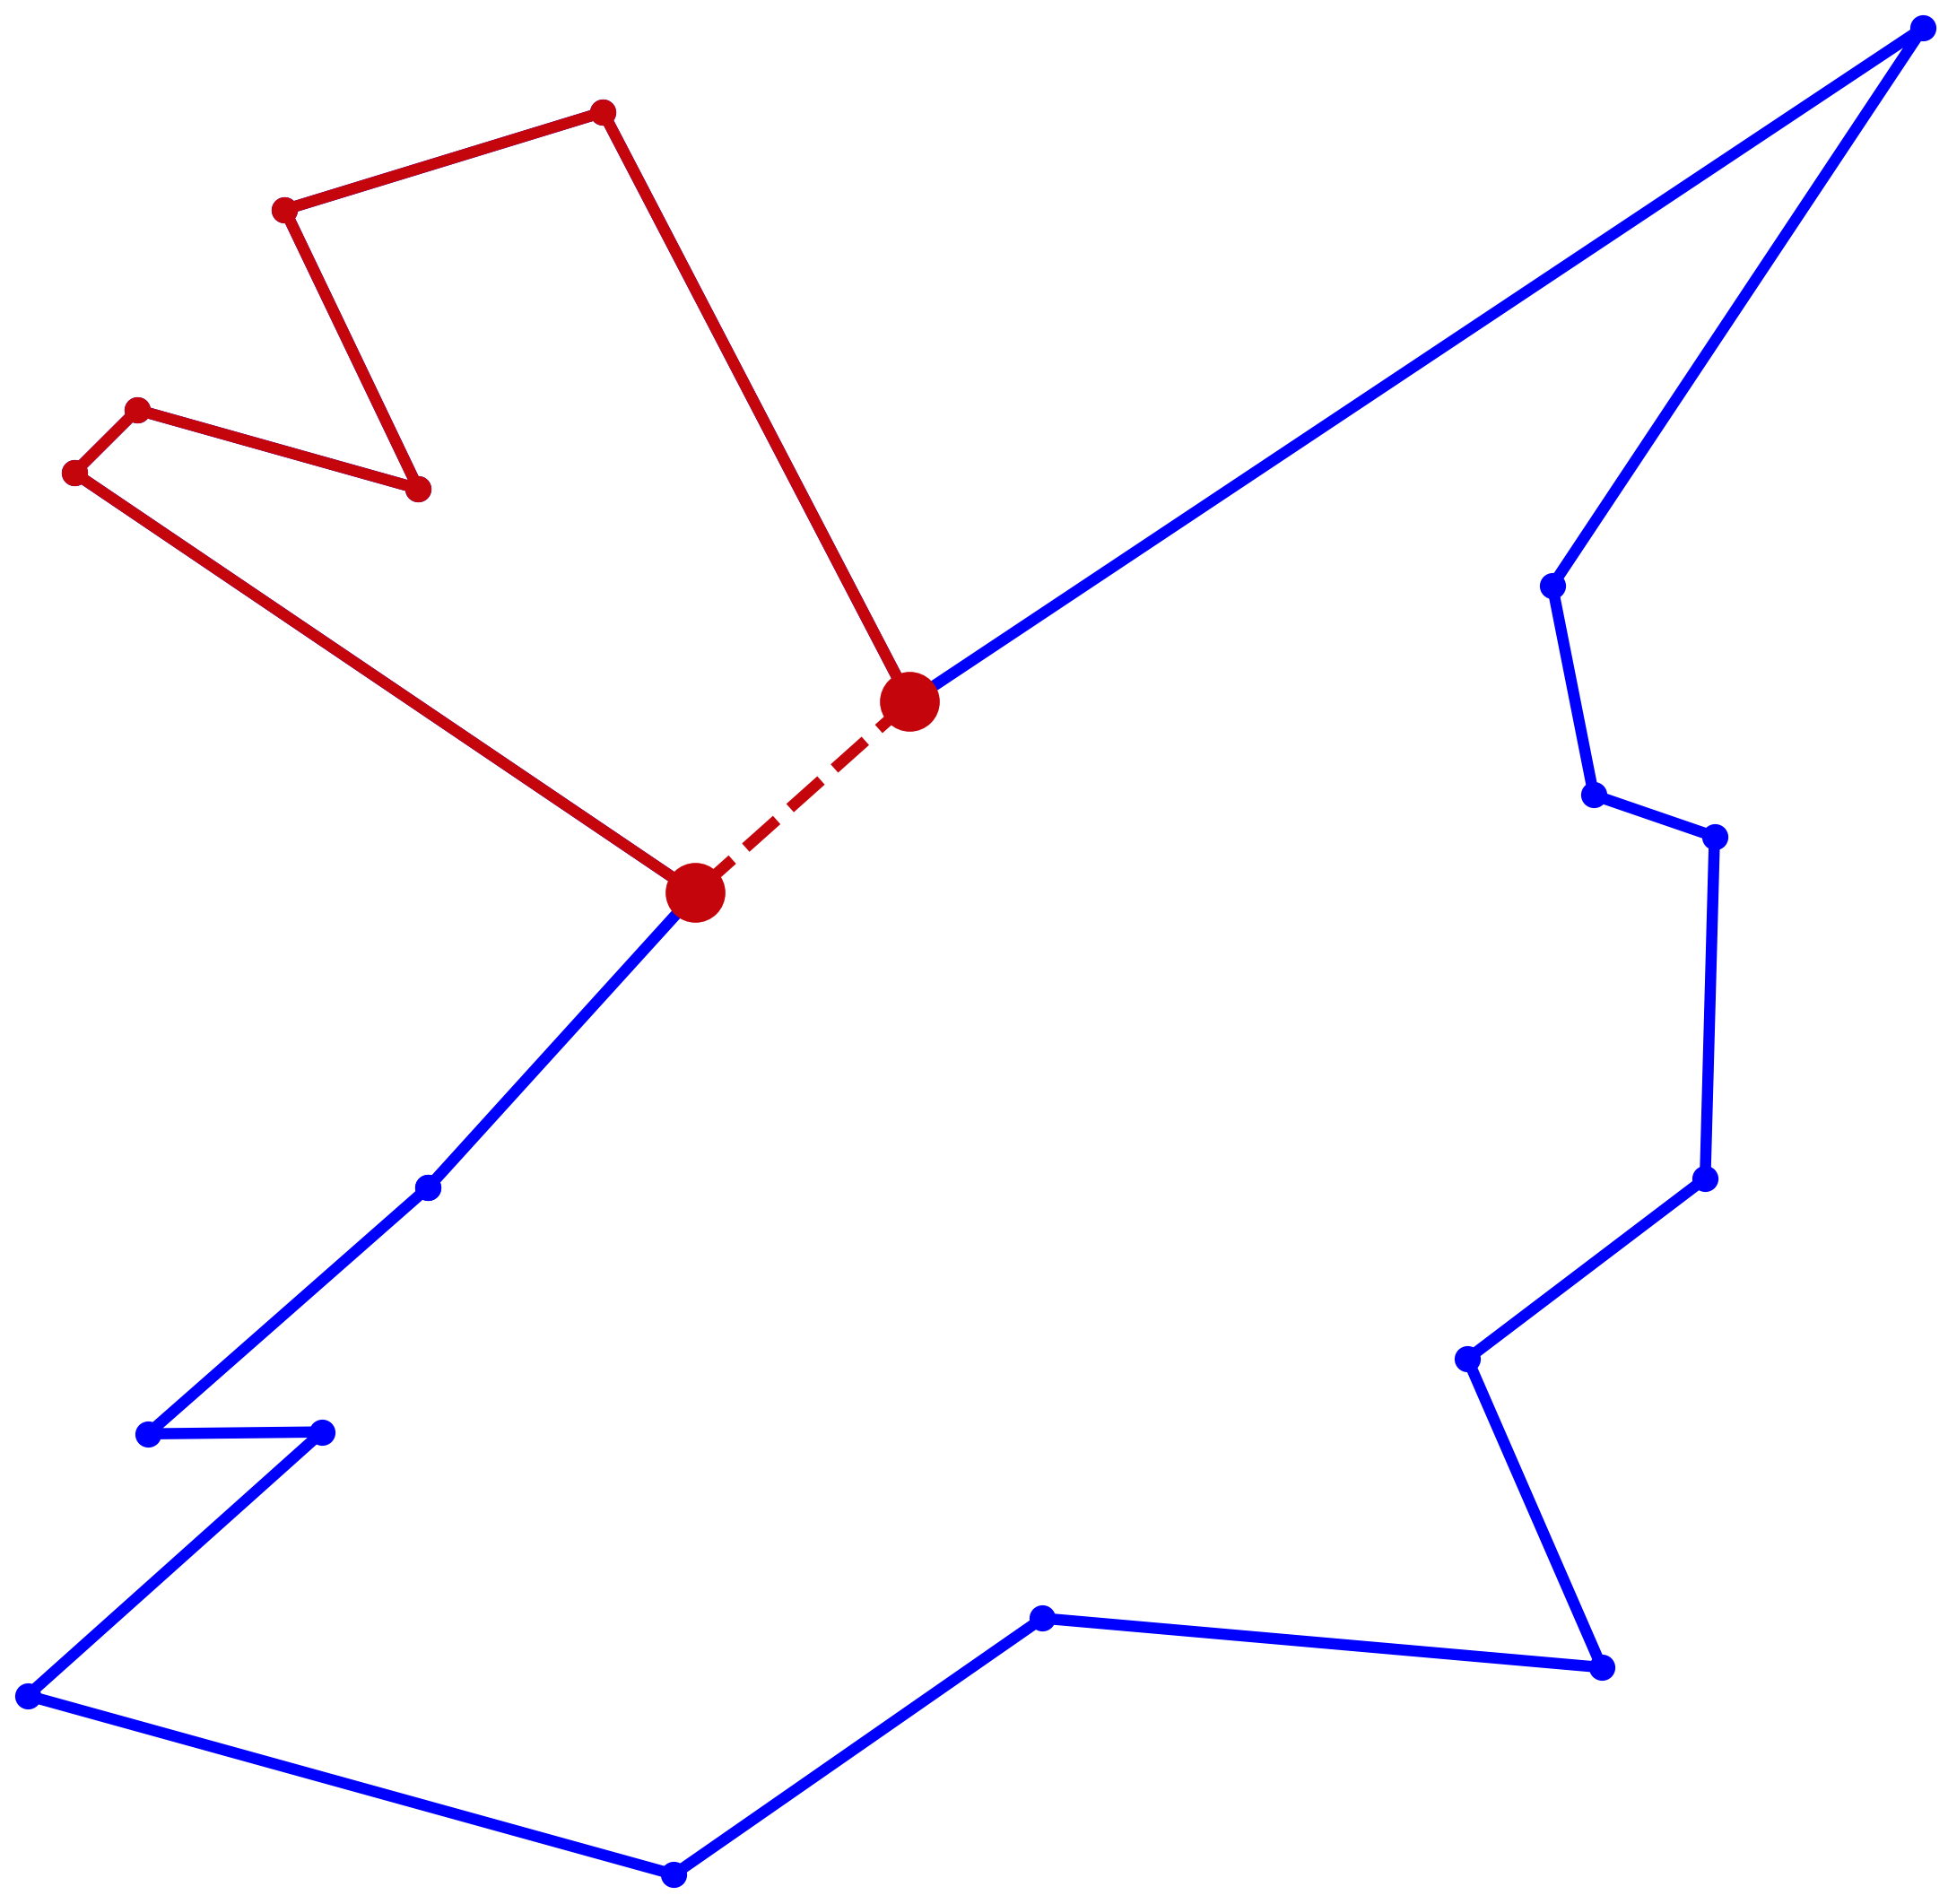
\includegraphics[width=0.75\textwidth]{figures/CA_def.png}
                \caption{Star-shaped}
                \label{fig:ca_def}
            \end{figure}
            \column{0.5\textwidth}
            \renewcommand{\thefigure}{1b}
            \begin{figure}
                \centering
                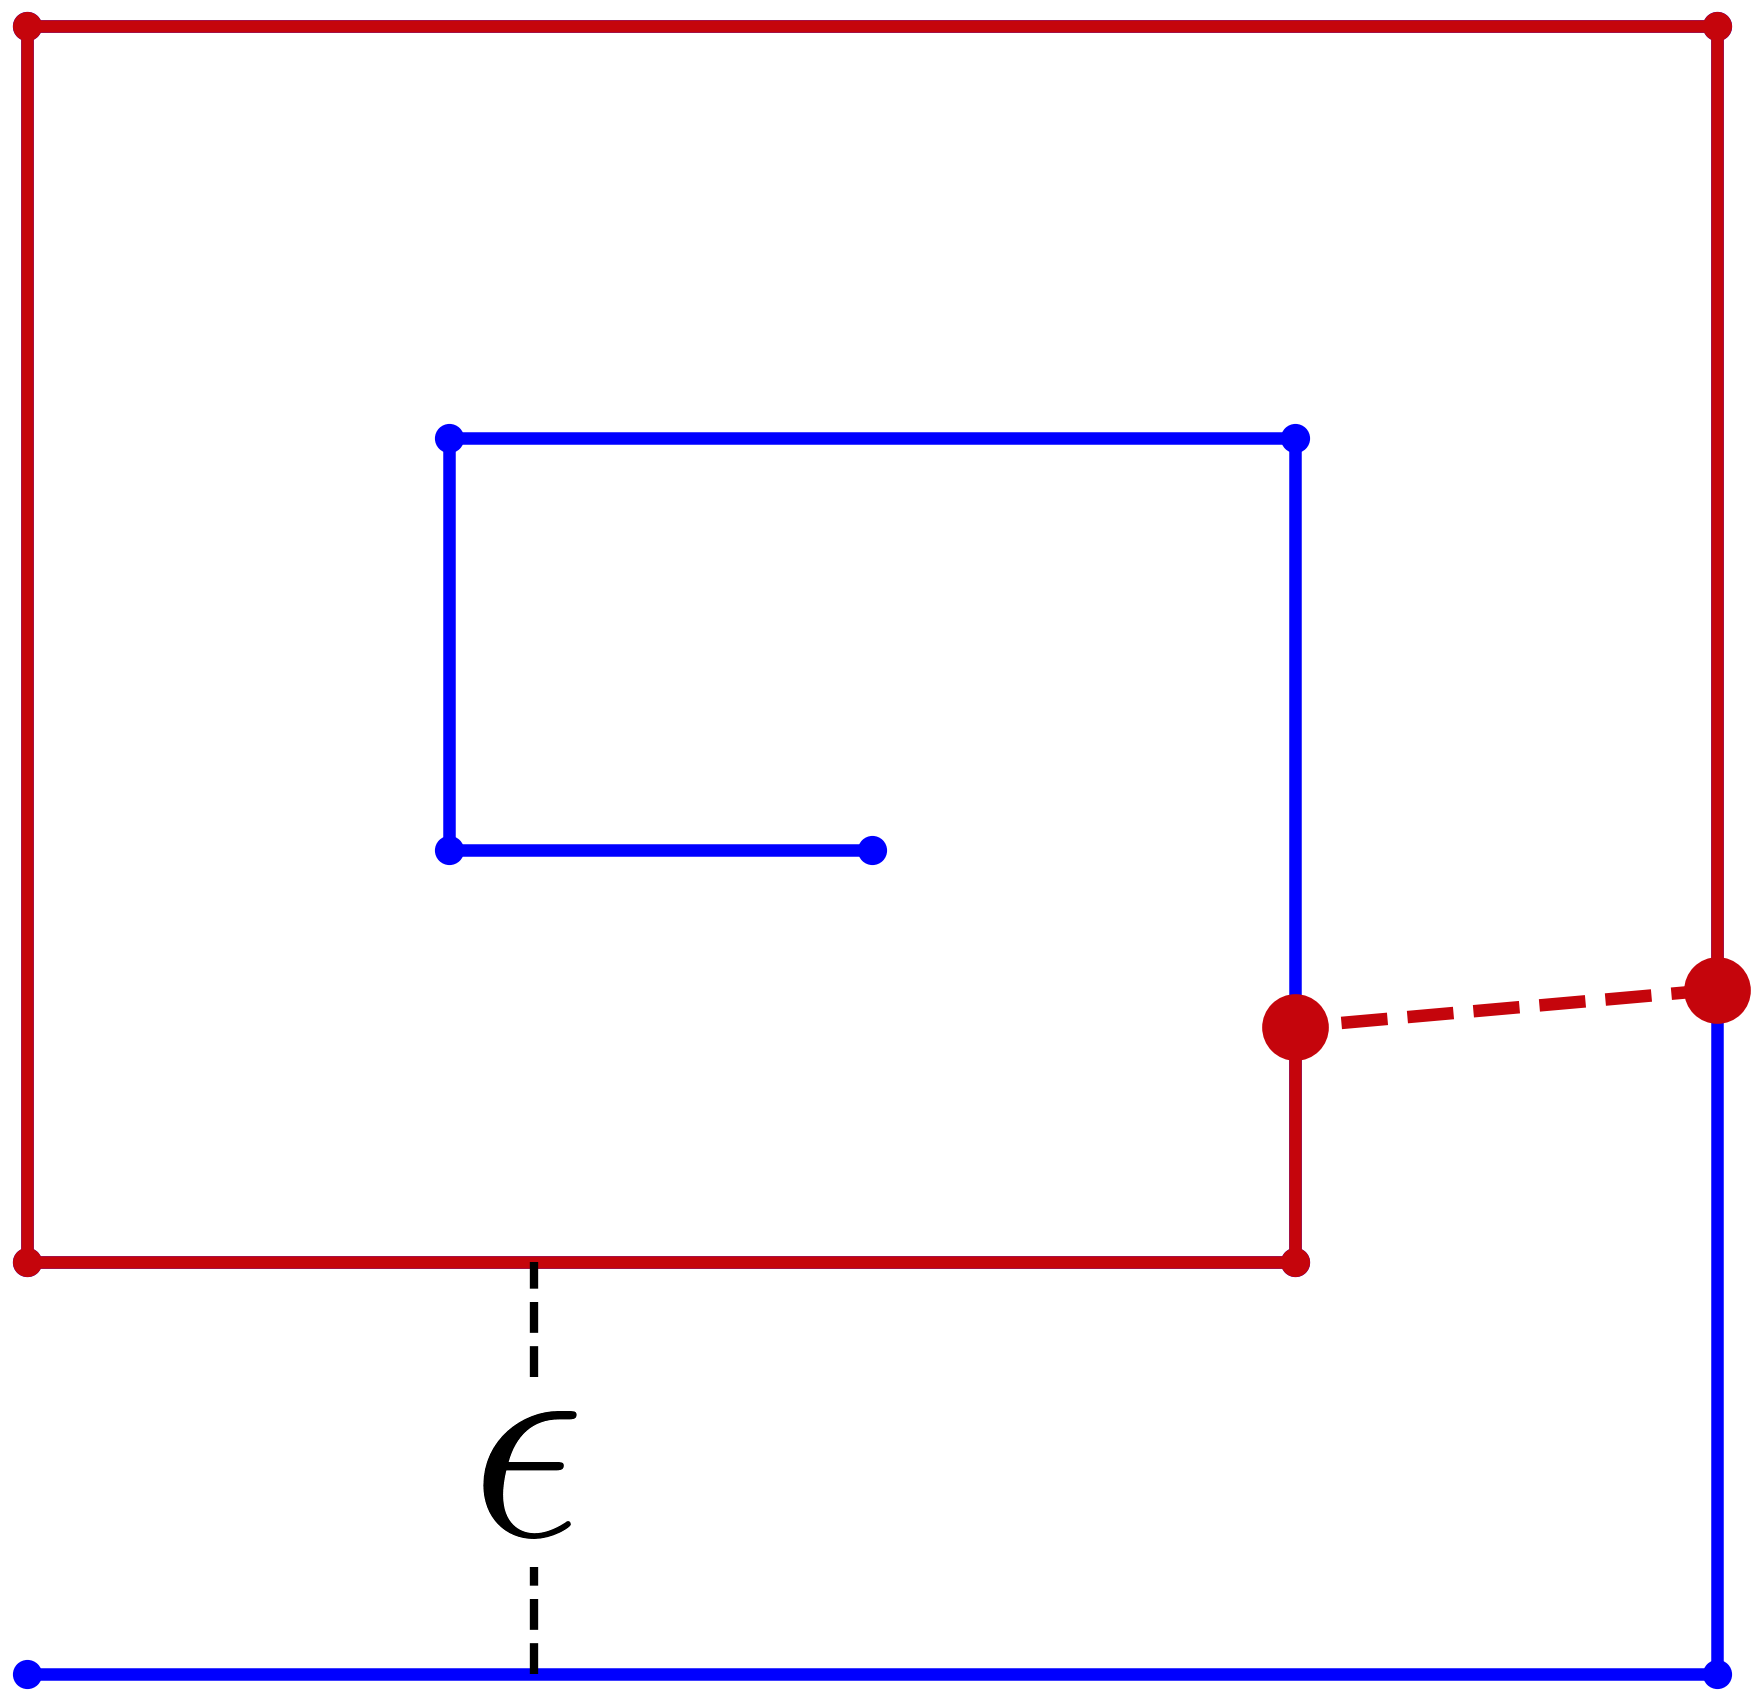
\includegraphics[width=0.75\textwidth]{figures/spiral.png}
                \caption{$\epsilon = 1/4$-spiral}
                \label{fig:spiral}
            \end{figure}
        \end{columns}
        \vspace{0pt}


    \column{0.35\textwidth}
        {\centering \large \textbf{Main Question} \\}
        
        How is the initial max speed of the vertices during expansion affected by the Chord-arc Constant?
        \vspace{1cm}
        \renewcommand{\thefigure}{2a}
        \begin{figure}
            \centering
            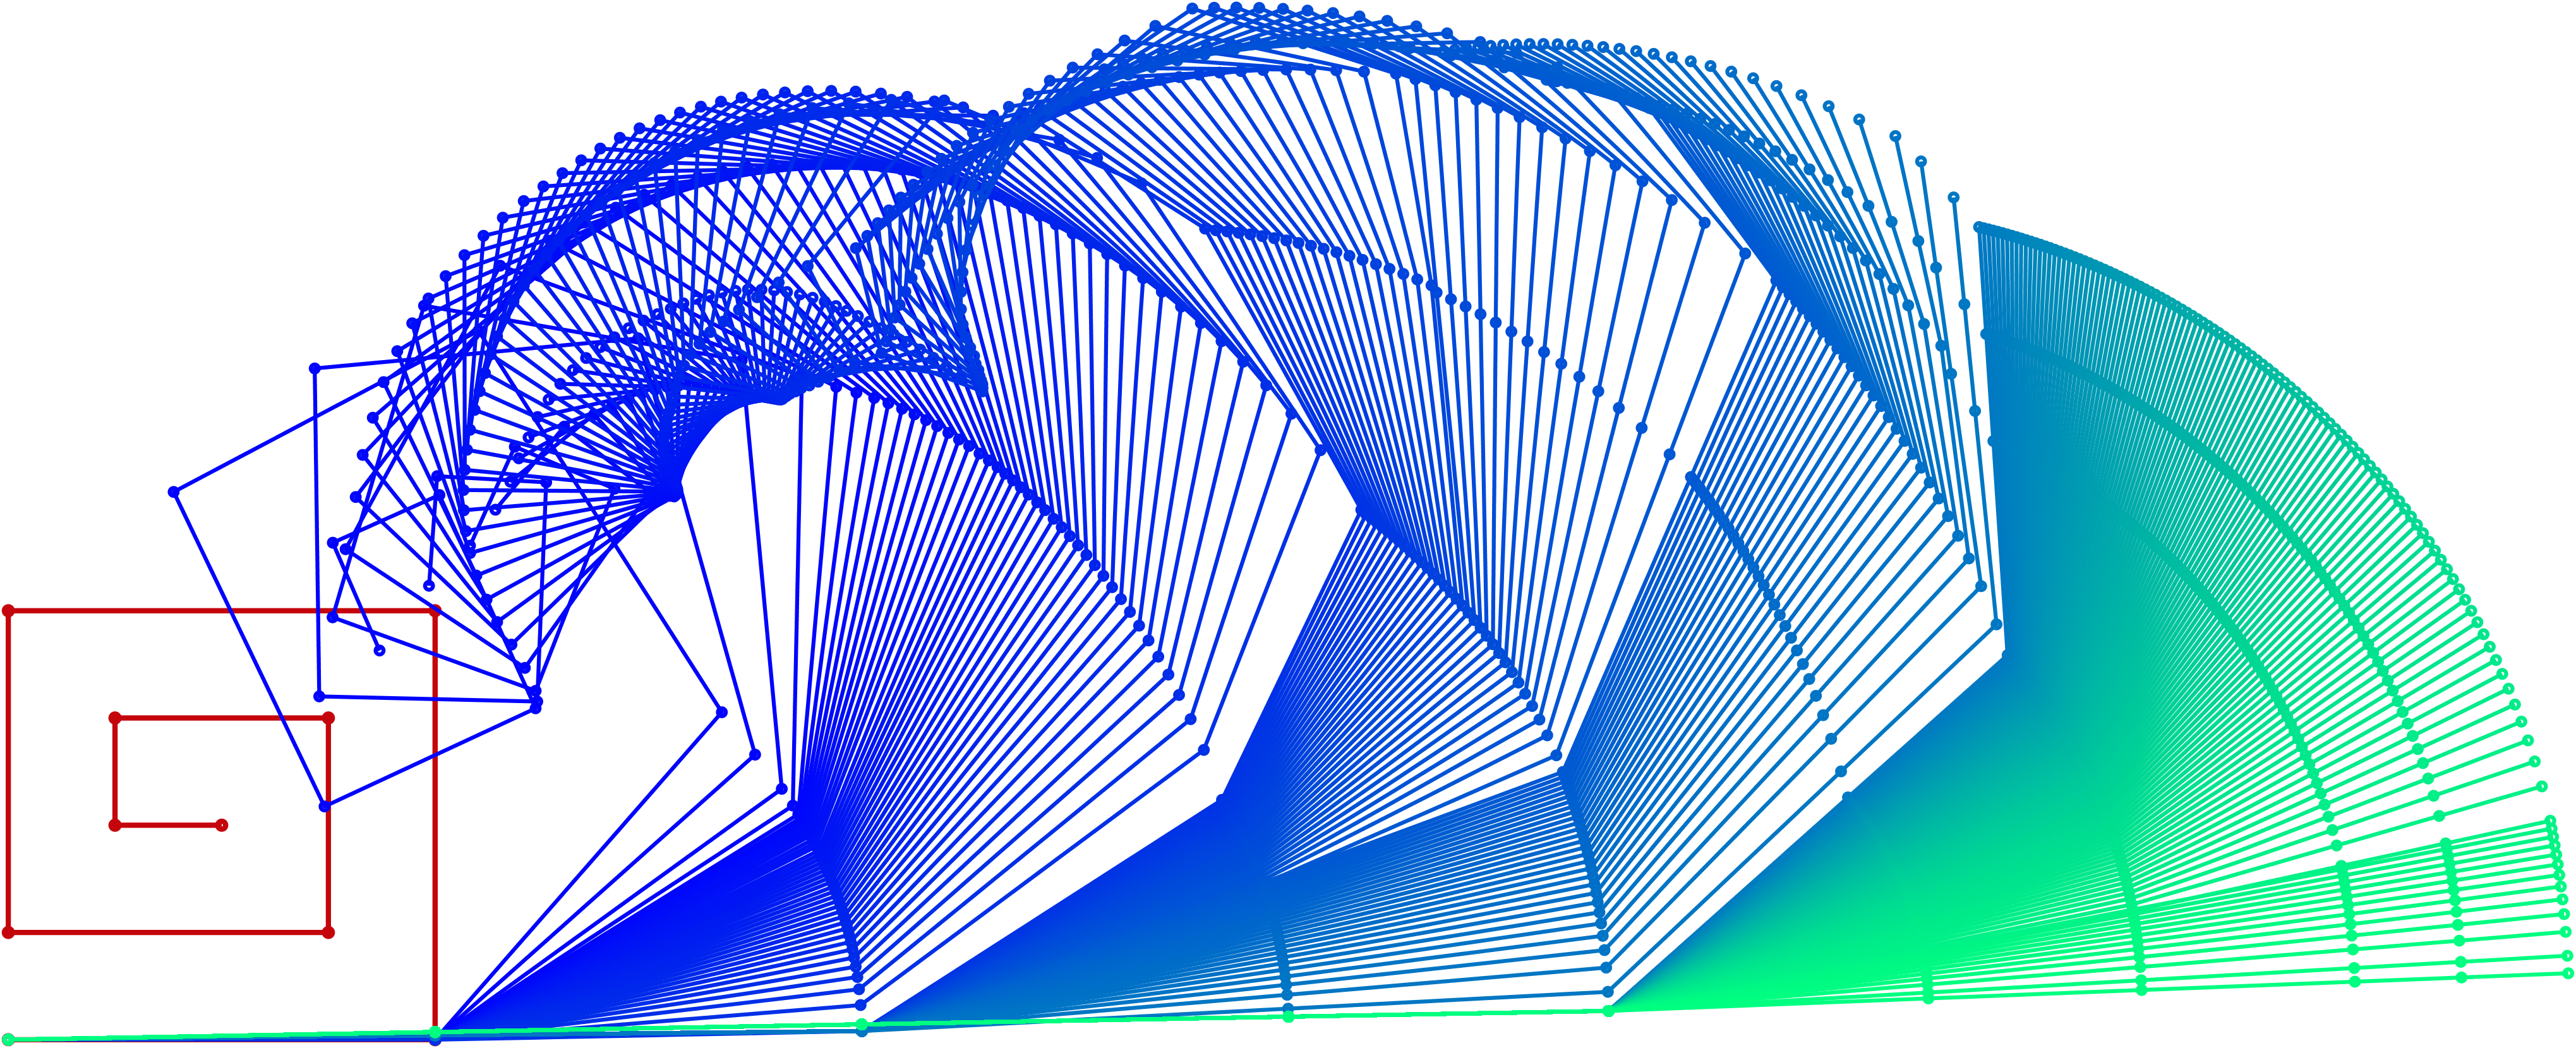
\includegraphics[width=0.8\textwidth]{figures/spiral_fourth.png}
            \caption{$\epsilon = 1/4$-spiral Expansion}
            \label{fig:spiral_exp}
        \end{figure}
        \vspace{-2cm}
        \renewcommand{\thefigure}{2b}
        \begin{figure}
            \centering
            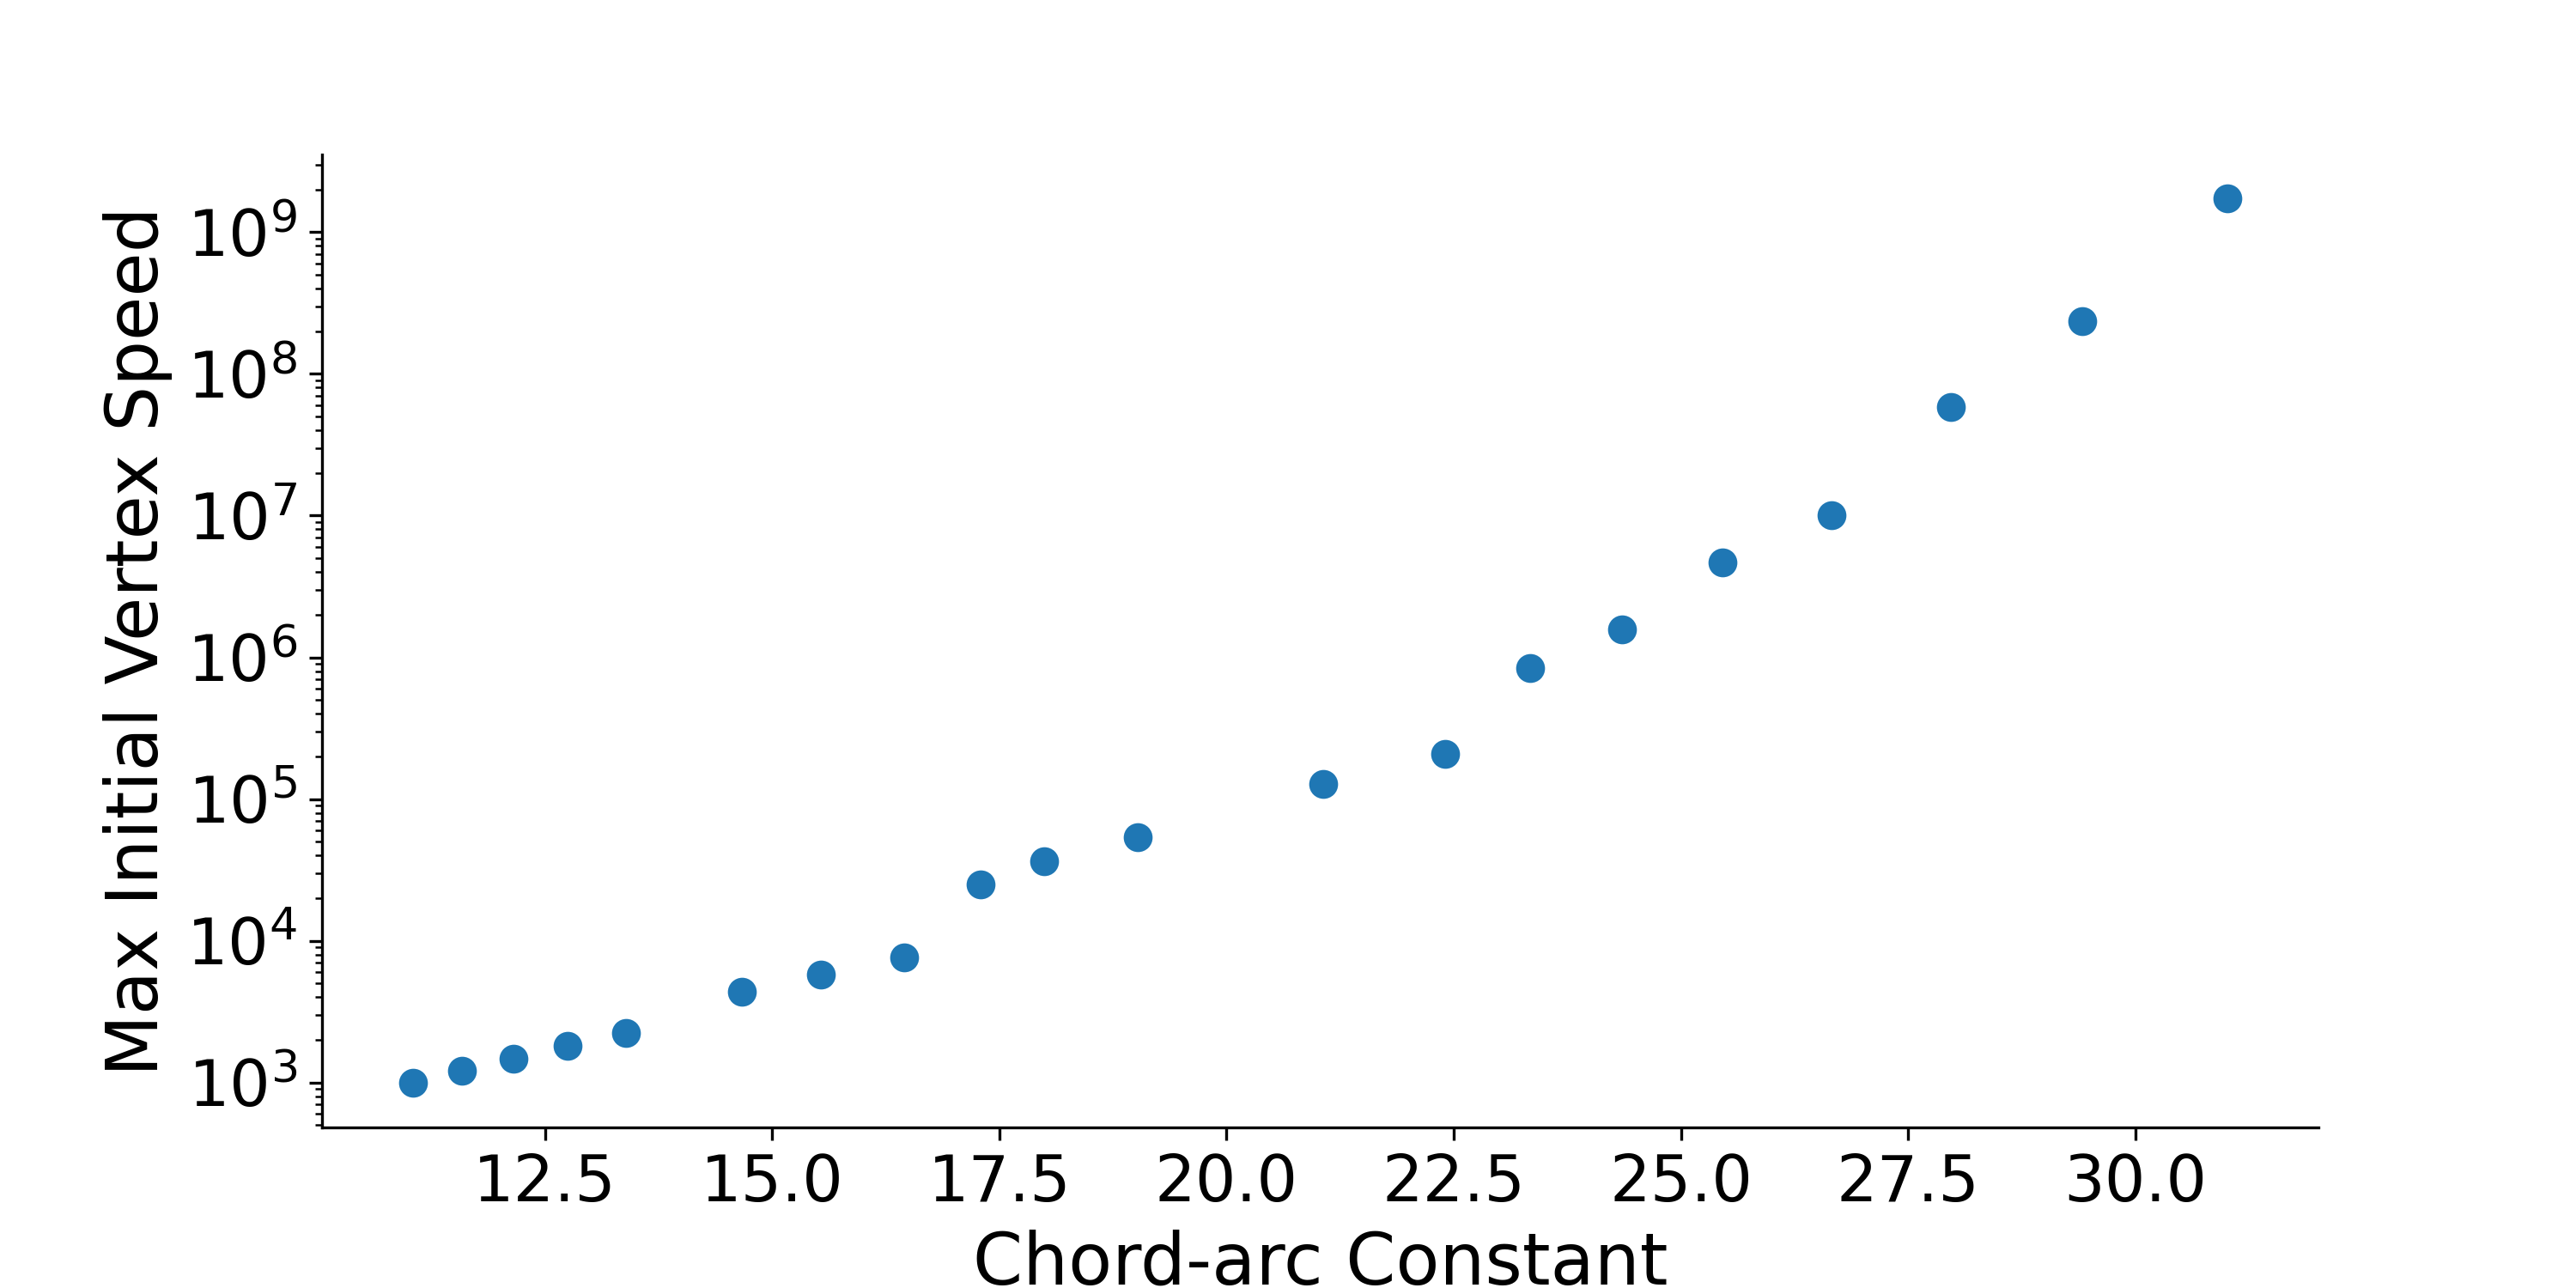
\includegraphics[width=\textwidth]{figures/scatter.png}
            \caption{Max Speed of $\epsilon$-spirals vs Chord-arc Constant}
            \label{fig:speed_v_chordarc}
        \end{figure}
        \vspace{-0.5cm}
        \renewcommand{\thefigure}{2c}
        \begin{figure}
            \centering
            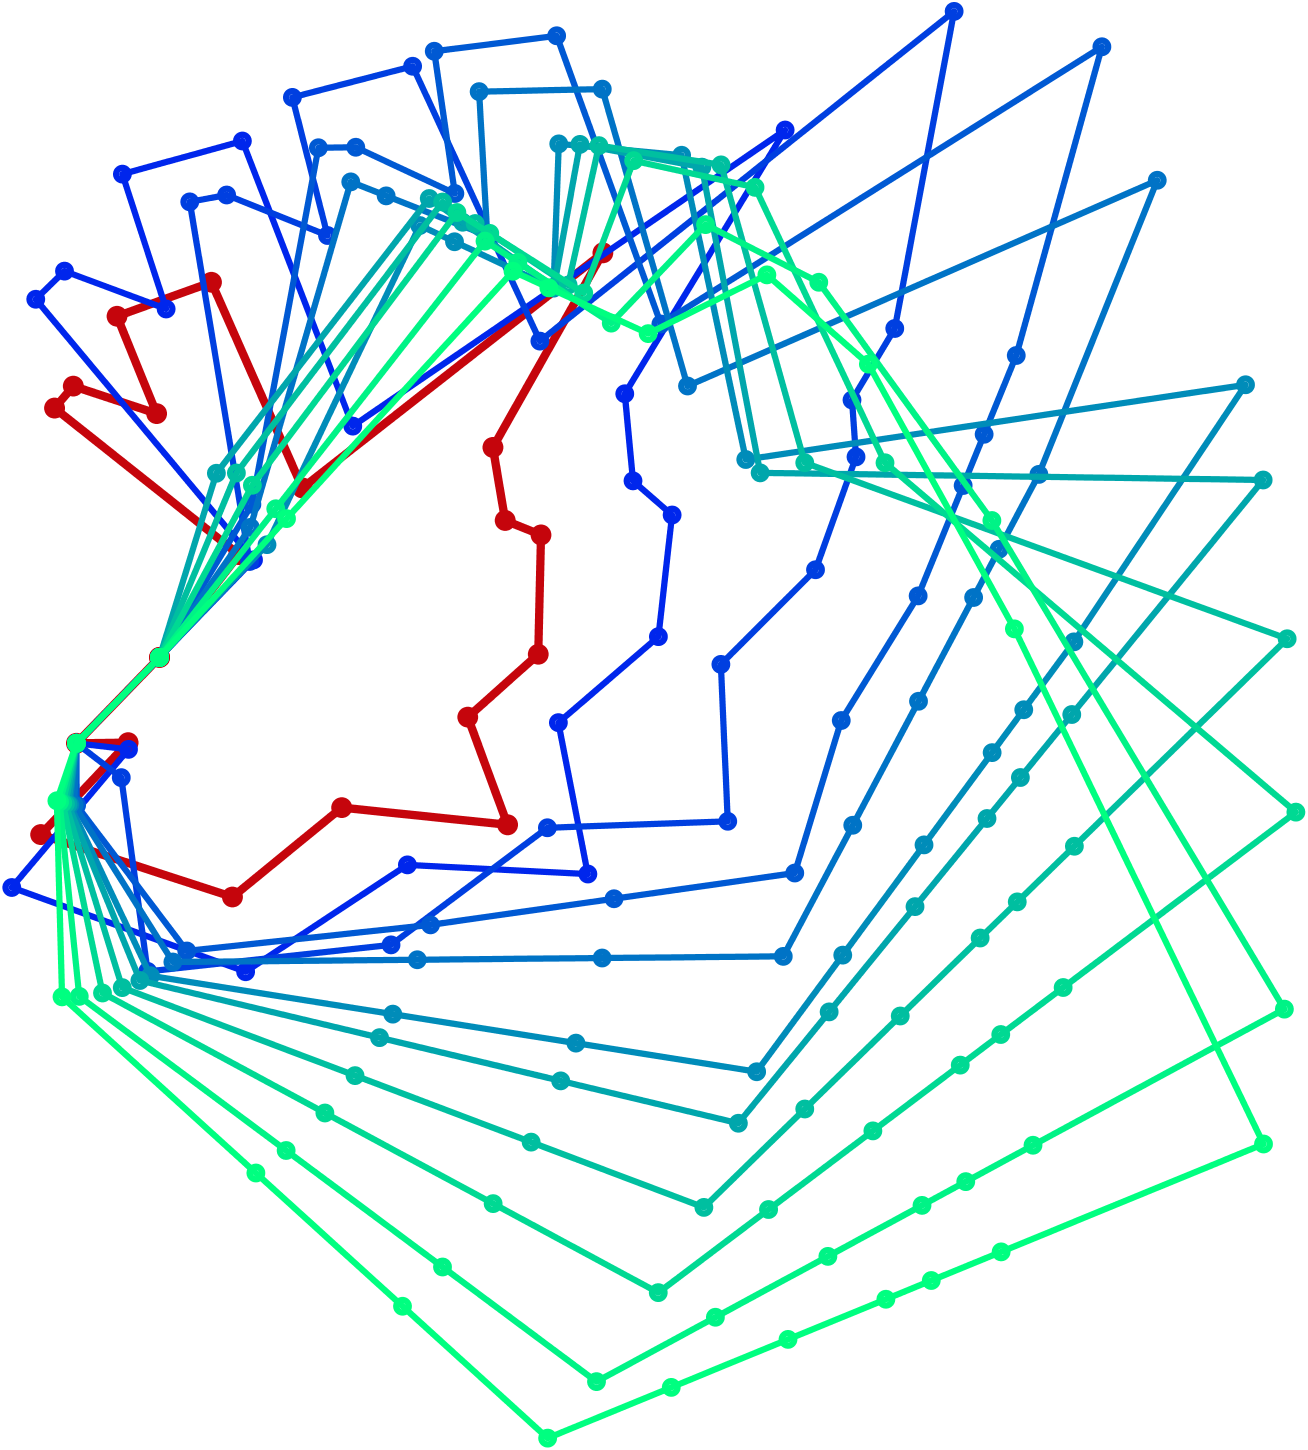
\includegraphics[width=0.36\textwidth]{figures/rand_poly.png}
            \caption{Star-shaped Polygon Expansion}
            \label{fig:star_exp}
        \end{figure}
        \vspace{0pt}
        
     % related questions   
    \column{0.3\textwidth}
        {\centering \large \textbf{Related Questions} \\}
        
        The Chord-arc Constant between two connected edges depends only on the angle $\theta$:
        \begin{columns}
            \column{0.4\textwidth}
            % \renewcommand{\thefigure}{3a}
            \begin{figure}
                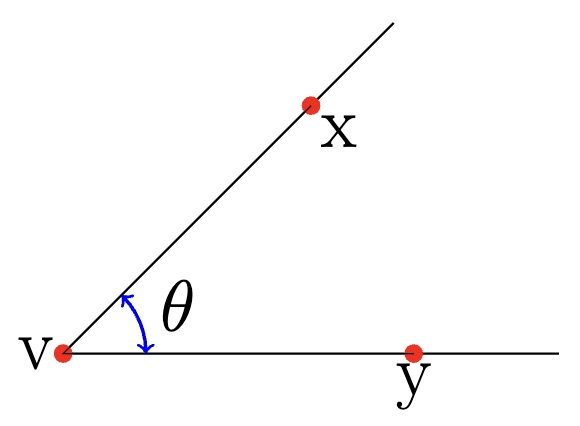
\includegraphics[width=1.1\textwidth]{figures/adj ca.jpg}
                \label{fig:adj_ca}
            \end{figure}
            \column{0.4\textwidth}
            Where $x$ and $y$ are equidistant to $v$.
            $$C_{adj}=\sqrt{\frac{2}{1 - \cos (\theta)}}.$$
        \end{columns}
        \vspace{-1.5cm}
        Elsewhere, finding the Chord-arc Constant is quite a computational challenge. We used optimization algorithms to find the maximizer $(a,b)^T$.
        \vspace{-1cm}
        \renewcommand{\thefigure}{3}
        \begin{figure}
            \centering
            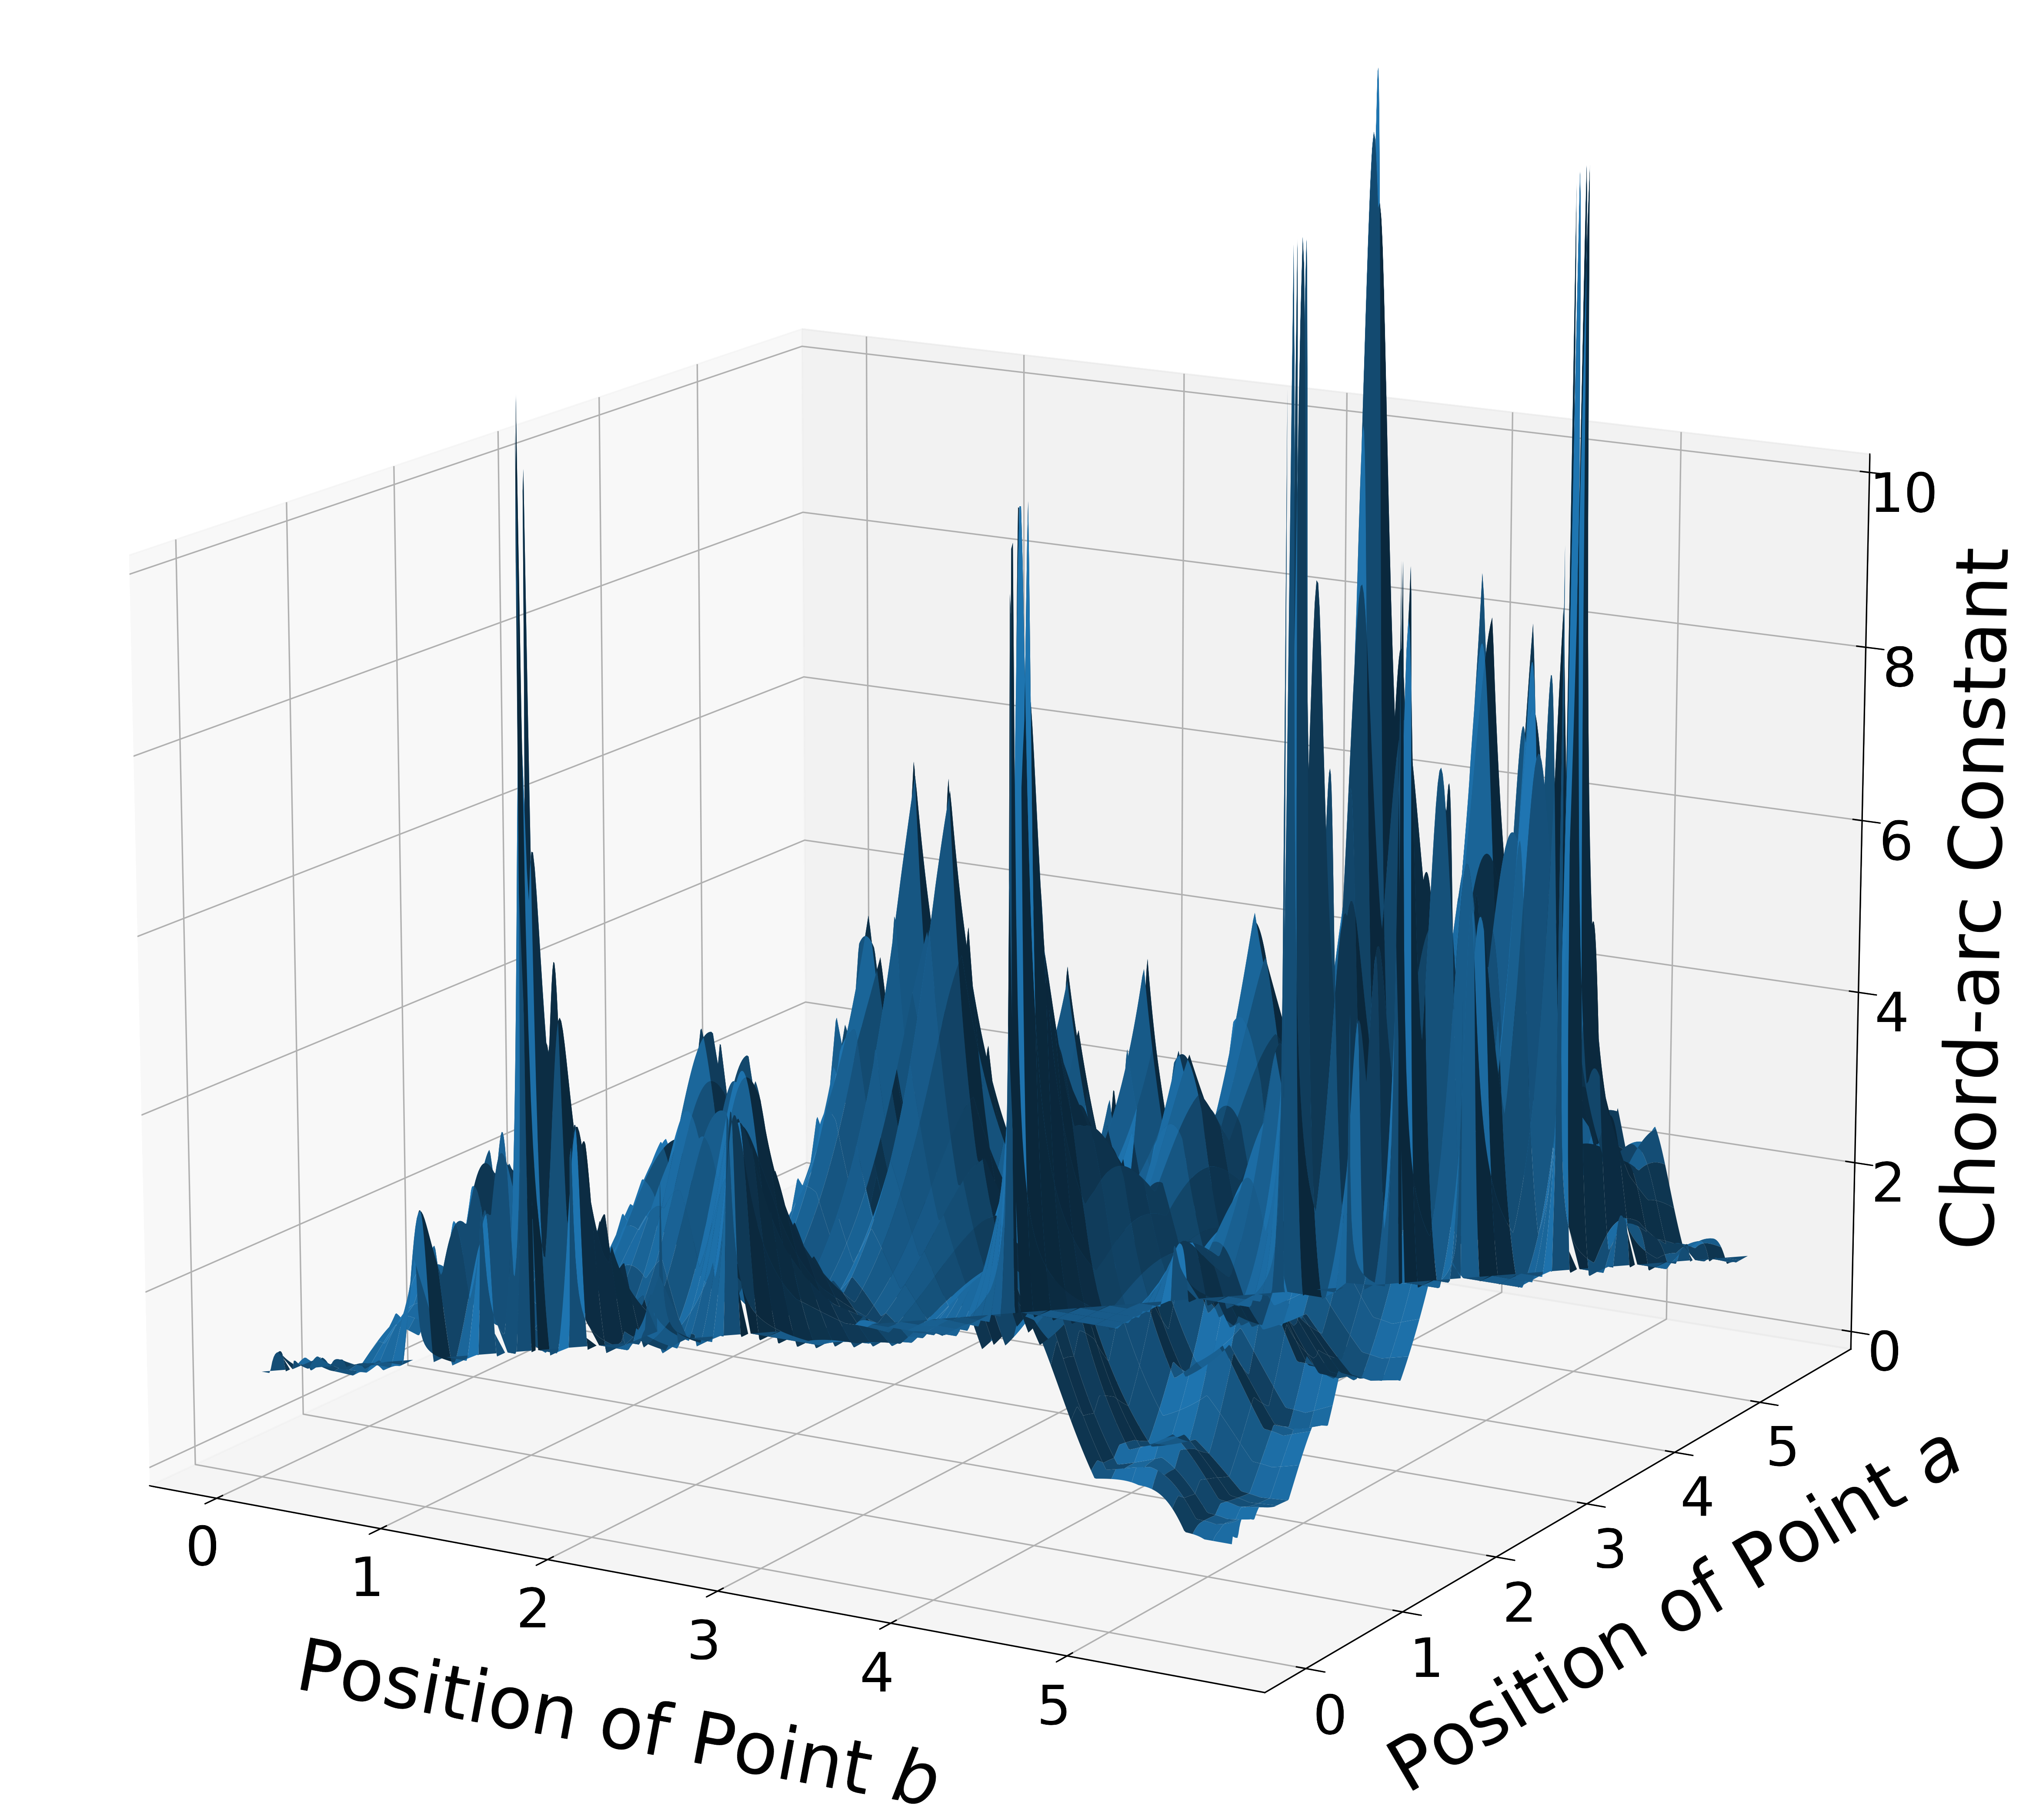
\includegraphics[width=0.83\textwidth]{figures/opt_3d.png}
            \caption{Chord-arc Constant Optimization}%A Vertex $v$ with Angle $\theta$ and Points $x$ and $y$ Equidistant to $v$}
            \label{fig:opt_3d}
        \end{figure}

        \textbf{Future Explorations:}
        \begin{enumerate}
            \item Efficiently calculating the Chord-arc Constant
            \item Other Carpenter's Rule Problem approaches
            \item Improving polygon generation algorithms
        \end{enumerate}
        \vspace{0pt}
    \end{columns}
    
        {
            \setbeamercolor{bibliography item}{fg=black}
            \setbeamercolor{bibliography entry author}{fg=black}
            \setbeamercolor{bibliography entry title}{fg=black}
            \setbeamercolor{bibliography entry note}{fg=black}
            \renewcommand*{\bibfont}{\tiny}
            \printbibliography
            \vspace{-1.3cm}
            \tiny
            Cheng, Ekman, Hu, and Lu were participants in an REU at UW-Madison in Summer 2022 which was supported by the National Science Foundation grants DMS-2037851, DMS-1653264, and DMS-2105580.
        }
\end{frame}
\end{document}